% -*- coding: utf-8 -*-
\section{QCM}

\paragraph{Question 1.} Quelle sont les coordonnées de la première composante principale des données décrites sur la figure~\ref{fig:pca_2d} ?
\begin{itemize}
\item[$\square$] $(1, 1)$
\item[$\square$] $\left(\frac{\sqrt{2}}{2}, \frac{\sqrt{2}}{2}\right)$
\item[$\square$] $(1, 0)$
\item[$\square$] $(\sqrt{2}, 0)$ 
\end{itemize}

\vspace{-160pt}
\begin{figure}[h]
  \centering
  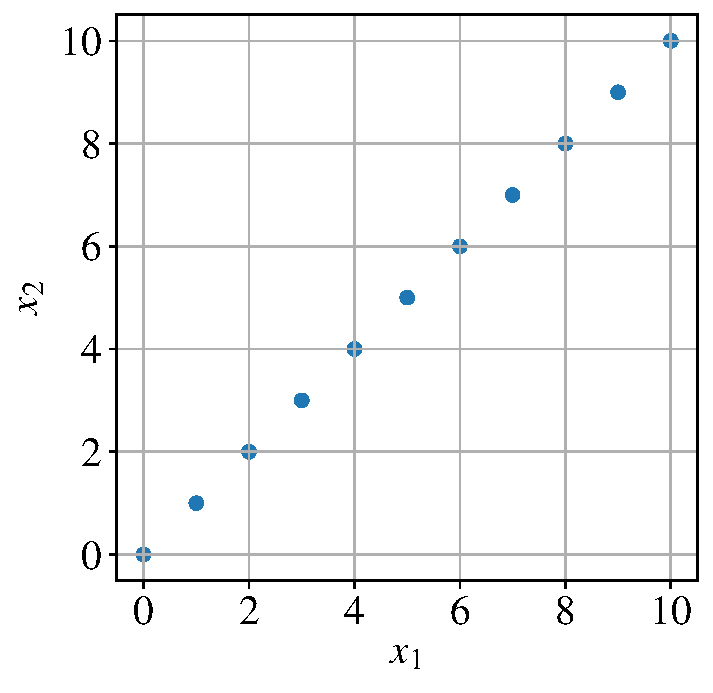
\includegraphics[width=0.4\textwidth]{figures/pca_2d}
  \caption{11 individus représentés par 2 variables $x_1$ et $x_2$.}
  \label{fig:pca_2d}
\end{figure}




\paragraph{Question 2.} Parmi les affirmations ci-dessous, lesquelles sont vraies ? On considère un jeu de données $X \in \RR^{n \times p}$ de $n$ individus en $p$ dimensions.
\begin{itemize}
\item[$\square$] La réduction de dimension relève de l'apprentissage supervisé.
\item[$\square$] La réduction de dimension relève de l'apprentissage non-supervisé.
\item[$\square$] La réduction de dimension facilite la visualisation des données.
\item[$\square$] L'analyse en composantes principales de $X$ permet de créer jusqu'à $n$ nouvelles dimensions. 
\item[$\square$] Les nouvelles variables créées par une analyse en composantes principales sont des combinaisons linéaires des $p$ variables.
\item[$\square$] L'analyse en composantes principales de $X$ s'obtient par une décomposition spectrale de $X$.
\item[$\square$] La sélection de variables consiste à conserver uniquement les variables dont la variance est la plus faible.
\end{itemize}

\section*{Solution}
{%
\noindent
\rotatebox[origin=c]{180}{%
\noindent
\begin{minipage}[t]{\linewidth}
\paragraph{Question 1.} La direction de plus grande variation des données est
la diagonale d'équation $x_1 = x_2$. Ainsi, la première composante principale
est le vecteur directeur de la diagonale, de norme 1, soit donc
$\left(\frac{\sqrt{2}}2, \frac{\sqrt{2}}2\right).$ \newline


\paragraph{Question 2.} 
\begin{itemize}
\item La réduction de dimension peut relever de l'apprentissage supervisé (par
  exemple, l'élimination des variables indépendantes de l'étiquette requièrent
  évidemment une étiquette) ou de l'apprentissage non-supervisé (par
  exemple, l'ACP). Elle est cependant souvent plutôt classée dans
  l'apprentissage non-supervisé car il s'agit d'analyse exploratoire des
  données et non pas d'analyse prédictive, ce qui peut prêter à confusion.
\item[\rlap{$\checkmark$}$\square$] La réduction de dimension facilite la visualisation des données.
\item[$\square$] L'analyse en composantes principales de $X$ permet de créer jusqu'à $n$ nouvelles dimensions. \\
FAUX, elle permet de créer jusqu'à $p$ nouvelles dimensions.
\item[\rlap{$\checkmark$}$\square$] Les nouvelles variables créées par une analyse en composantes principales sont des combinaisons linéaires des $p$ variables.
\item[$\square$] L'analyse en composantes principales de $X$ s'obtient par une décomposition spectrale de $X$.\\
FAUX, il s'agit de la décomposition spectrale de $X^\top X$.
\item[$\square$] La sélection de variables consiste à conserver uniquement les variables dont la variance est la plus faible. \\
FAUX, \textit{une des techniques} de sélection de variables consiste à \textit{éliminer} les variables dont la variance est la plus faible. \\
\end{itemize}
\end{minipage}%
}%



%%% Local Variables:
%%% mode: latex
%%% TeX-master: "../../sdd_2025_poly"
%%% End:
